\documentclass{CUP-JNL-DTM}%

%%%% Packages
\usepackage{graphicx}
\usepackage{multicol,multirow}
\usepackage{amsmath,amssymb,amsfonts}
\usepackage{mathrsfs}
\usepackage{amsthm}
\usepackage{rotating}
\usepackage{appendix}
\usepackage[numbers]{natbib}
\usepackage{ifpdf}
\usepackage[T1]{fontenc}
\usepackage{newtxtext}
\usepackage{newtxmath}
\usepackage{textcomp}
\usepackage{xcolor}
\usepackage{lipsum}
\usepackage[colorlinks,allcolors=blue]{hyperref}

\newtheorem{theorem}{Theorem}[section]
\newtheorem{lemma}[theorem]{Lemma}
\theoremstyle{definition}
\newtheorem{remark}[theorem]{Remark}
\newtheorem{example}[theorem]{Example}
\numberwithin{equation}{section}

\newcommand{\Julia}{\texttt{Julia} }

% \usepackage{lineno}
% \linenumbers

%\jname{Physics/Math}
\articletype{CAPSTONE PROJECT}
%\artid{20}
%\jyear{2022}
%\jvol{}
%\jissue{}
%\raggedbottom


\begin{document}

\begin{Frontmatter}

\title[Article Title]{Using Scientific Machine Learning to solve Partial Differential Equations}

\author[1]{Miles Cochran-Branson}\orcid{0000-0002-8514-4315}
% \author[2]{Author Name2}\orcid{0000-0001-8823-831X}
% \author[2]{Author Name3}\orcid{0000-0002-0251-345}

\authormark{M. Cochran-Branson}

\address[1]{\orgdiv{Department of Physics and Mathematics}, \orgname{Lawrence University}, \orgaddress{\city{Appleton}, \state{WI}}}%, \postcode{54911}, \country{USA}}}

%\address[2]{\orgdiv{Division}, \orgname{Organization}, \orgaddress{\city{City}, \postcode{Pincode}, \state{State},  \country{Country}}. \email{name2@email.com}}

\keywords{SciML, Scientific Computing, ML/AI, PINN, PDEs}

\abstract{Machine learning and artificial intelligence have been used with huge success in data science, mathematics, and physics as well as numerous other fields to solve complex or previously impossible computational problems. Computationally intensive problems in physics such as data analysis using a complex model and little data, or finding numerical solutions to differential equations have traditionally been solved with classical scientific computing techniques such as Taylor-series expansions or approximations using polynomials. Recent efforts have gone into replacing these techniques with neural networks and machine learning. Neural networks have the potential to fit any complex model or differential equation solution very accurately and can solve these problems quickly. In the following paper, I describe the basic principles of the growing field of Scientific Machine Learning (SciML). I will use the techniques I describe to solve the Einstein field equations to obtain the Schwarzschild metric using the package \texttt{NeuralPDE.jl} in the \Julia programming language. This example demonstrates the power a physics-informed neural network has in solving large, highly coupled, systems of partial differential equations. }

\end{Frontmatter}

\localtableofcontents

%% ---------------------------------------------------------------
%% Text Body!!

\section{Introduction}

Machine learning and scientific computing are two prominent fields with applications in physics, mathematics, and computer science. An initiative laid out by the DOE in 2019 outlines the importance and potential of the ever growing field of SciML \cite{bakerWorkshopReportBasic2019}. In this report, they indicate the challenges that SciML could potentially solve: lack of data in analysis, and solving differential equations. In the first case, in problems where data is either expensive or impossible to collect, implementations of machine learning become impossible. This can be overcome if we can incorporate physics knowledge of the system into the neural network. Such implementations make use of \emph{Physics-Informed Neural Networks} (PINN) \cite{karniadakisPhysicsinformedMachineLearning2021}. It turns out that PINN can also solve differential equations by slight modification of the process used above. In fact, we can include data into solving of differential equations to better fit a model or aid in solving the equation(s). 

Below, I will describe how machine learning in tandem with scientific computing can solve both of these problems elegantly and efficiently. I will begin by outlining the basics of what machine learning is in section two. In sections three and four I will describe how to solve ODEs and PDEs with Physics-Informed Neural Networks (PINN). Finally, in section five I present a specific problem: solving Einstein's field equations to obtain the Schwarzschild Metric using the \Julia library \texttt{NeuralPDE.jl}. In the conclusions section I describe some future directions of this research and hopefully some suggestions? We shall see. 

\section{Machine Learning}

Machine learning and artificial intelligence are prominent features of our everyday life from personalized advertisements to facial recognition software. Machine learning is also a powerful analytical tool in scientific research, in particular with model development and validation. Below, I will describe how neural networks can be trained to make predictions and give some motivation for why neural networks are well suited for function approximation. 

\subsection{Neural Networks}

A neural network is simply a function composed of layers of matrix multiplication. As input, a neural networks take a matrix with size of number of obervables by number of data points and gives as an output a vector of weights. Thus, our network takes the form

\begin{equation}
    f : \mathbb{R}^{n\times m} \rightarrow \mathbb{R}^{\ell}
\end{equation}
where $n$ is the number of parameters for each data point $m$ and $\ell$ is the number of desired output features. Networks have a fixed size defined by the number of \emph{hidden layers} and the number of \emph{nodes} each hidden layer has. 

\begin{figure}
\centering
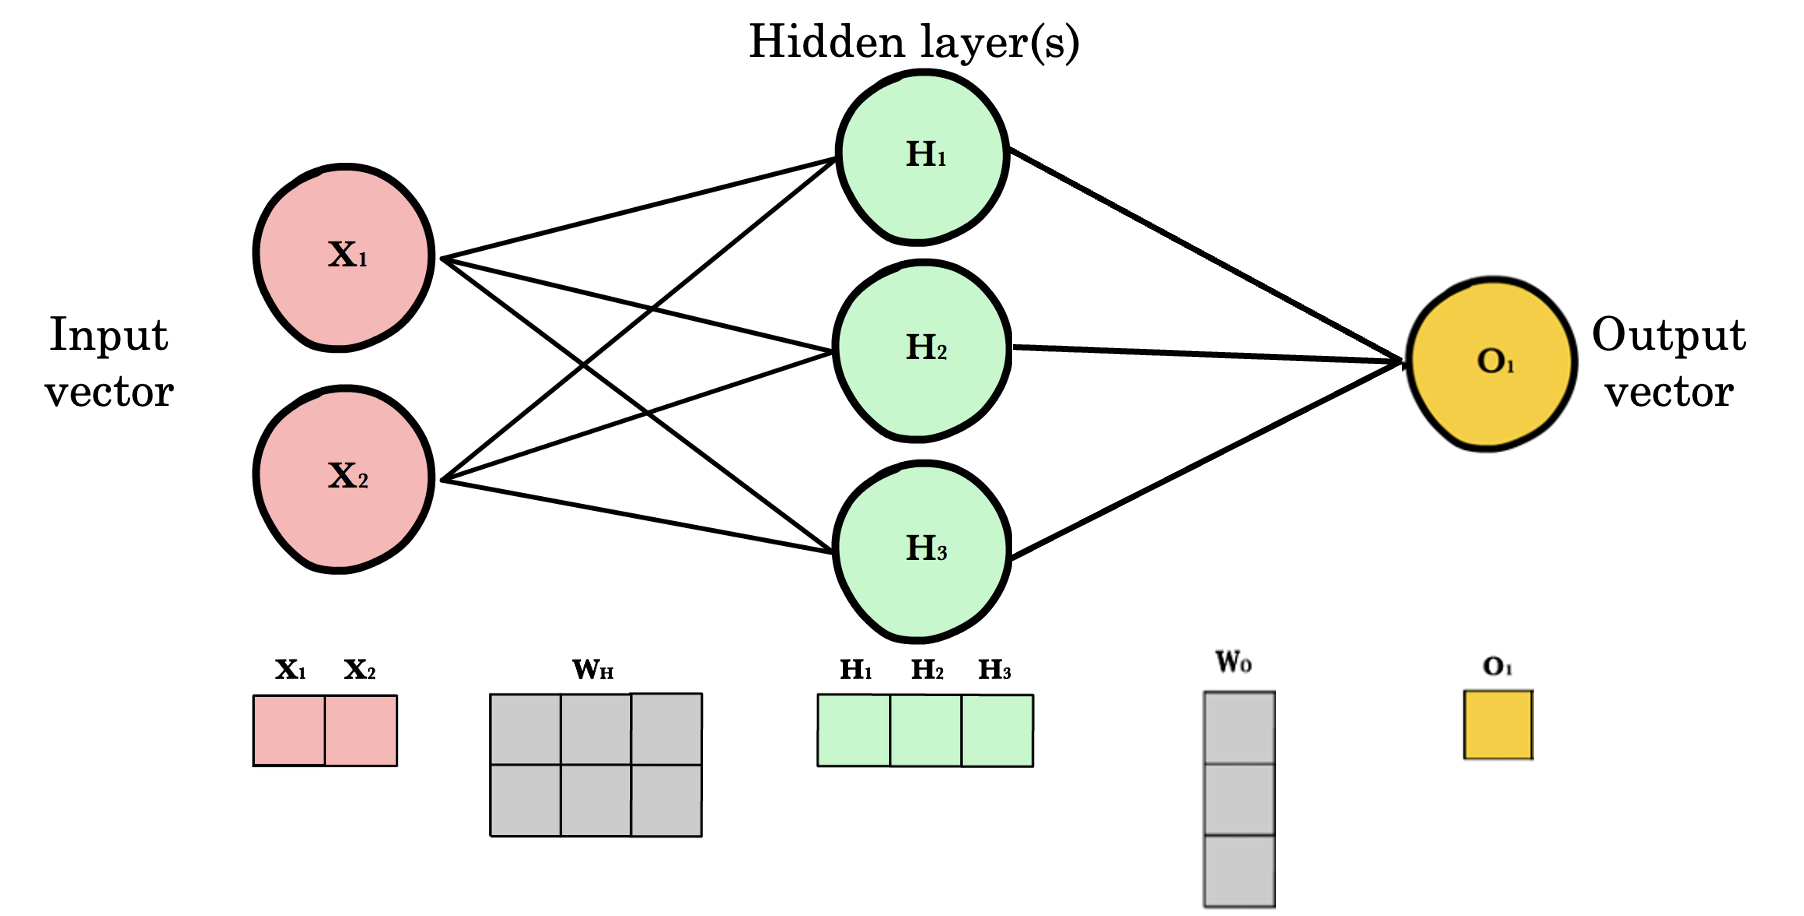
\includegraphics[width=0.7\linewidth]{figures/NN_example.png}
\caption{An example of a simple neural network with two inputs, one hidden layer with three nodes, and a single output. The network is defined by the weights connecting the layers which are represented as matrices. At each node, the weights are passed to a function called the \emph{activation function} which scales the weights appropriately. In principle, the size of the network can change in every dimension. }
\label{fig:NNexample}
\end{figure}

Hidden layers cannot be directly accessed in the training process and are thus so named. A node within a layer describes a connection point between layers. Connections are achieved via a multiplication by a weight stored in the network. Modification of these weights changes the way in which nodes are connected to each other and thus how inputs are interpreted by the network. At each node, the weight passed to the node is modified by an \emph{activation function}. These typically modify the weight such that each weight is not linearly connected to each other. This allows us to describe a more complex input space more accurately \cite{dubeyActivationFunctionsDeep2022}. Some examples of activation functions include the sigmoid defined by 

\begin{equation}
    \sigma(w) = \frac{1}{1 + e^{-w}},
\end{equation}
$\tanh(w)$, and LSTM defined by $f(w) = \textrm{max}\{0,x\}$ where in each case $w$ is the weight provided by the previous layer. In the work that follows, we typically use a sigmoid activation function. 

An example of a simple neural network with one hidden layer is shown in Fig. \ref{fig:NNexample}. This network has one input dimension and, as shown in the graphic, we feed one data point $X$ with two features $x_1, x_2$ into the network. Parameters of the network are stored in the matrix $W_0$ such that when we do the multiplication $X W_0$ we get a vector of three values corresponding to the three nodes of the single hidden layer. The activation function is now applied to these values. We then multiply by the weights $W_1$ to get our output of a single value which is passed to one final activation function. In most cases, the activation in the final node is the identity function $f(x) = x$. Notice that we can have as many inputs, layers, nodes, and output nodes as we would like. Scaling up the amount of hidden layers will increase the weights of the matrix significantly. 

Now that we have built some neural network, we would like to have it make some useful predictions! This involves picking some special set of weights through a process called training. 

\subsection{Training Neural Networks}

\subsection{The Universal Approximation Theorem}

Thang that makes everything work!

\begin{theorem}

Consider $x \in \Omega$ and let $u(x)$ be a regular function and $N(x,w)$ be a neural network with weights $w$. Then we can find some arbitrarily small $\epsilon \in \Omega$ such that 

\begin{equation}
	||N(x,w) - u(x)|| < \epsilon. 
\end{equation}

\end{theorem}

\section{Solving ODEs with Physics-Informed Neural Networks}

\section{Solving PDEs with Physics-Informed Neural Networks}

We now turn out attention to solving partial different equations using techniques from scientific machine learning. We will use the package \texttt{NeuralPDE.jl} \cite{zubovNeuralPDEAutomatingPhysicsInformed2021} to solve some examples. 

Consider a partial differential equation given by 

\begin{equation}
	f(u(x); \lambda) = 0
\end{equation}
where $x \in \Omega$ are the independent variables in the space $\Omega$, $u(x)$ is the solution, $f$ is some non-linear function acting on $u$ and $\lambda$ are the parameters of the equation. To solve with a neural network $N(x, w)$ where $N$ is a neural network with weights $w$, we want to fulfill 

\begin{equation}
	f(N(x, w); \lambda) \approx 0.
	\label{eqn:NNapprox}
\end{equation}
The universal approximation theorem tells us that this should be possible. The error of the above equation is then given by 

\begin{equation}
	L(w) = \int_{\Omega} ||f(N(x,w); \lambda)||\,dx. 
	\label{eqn:NNloss}
\end{equation}
We have suggestively named the error $L$ as we can use this function as a loss function in training our neural network $N$ by attempting to minimize $L$. Our computational problem then reduces to the problem of evaluating the integral in Eqn. \ref{eqn:NNloss}. Notice that in practical problems, we apply boundary conditions $b_i$ on $\partial \Omega \in \Omega$. In order to use these in our neural network, we add in these conditions to our loss function giving us 

\begin{equation}
	L(w) = \sum_i\int_{\Omega\setminus\partial\Omega} ||f_i(N(x,w); \lambda)||\,dx + \sum_i\int_{\partial\Omega} ||b_i(N(x,w); \lambda)||\,dx.
	\label{eqn:complete_loss} 
\end{equation}
where we have generalized the problem to a system of coupled differential equations $f_i$. 

There are several different methods for evaluating the above integral namely: grid approximation techniques, stochastic grid approximation techniques, and machine learning (quadrature) techniques. A simple grid approximation takes the space $\Omega$ and divides it into units of volume $\Delta V$ with a specific length. The PDE is evaluated at each of this points and scaled by the volume, thus our integral is computed via 

\begin{equation}
	\int_{\Omega} ||f(N(x,w); \lambda)||\,dx = \sum_i \Delta V ||f(x_i)||.
\end{equation}
This method has two main disadvantages: 1) as the dimension of the problem increases, the number of points we sample increases exponentially in order to maintain the same granularity and 2) no evaluation of the integral is done between grid points, thus information can be quickly lost. To solve the second problem, we can use stochastic methods of sampling---i.e., use Monte Carlo techniques to evaluate the integral. This can be described by 

\begin{equation}
	\int_{\Omega} ||f(N(x,w); \lambda)||\,dx = \alpha \sum_i ||f(x_i)||.
\end{equation}
for some scaler $\alpha$. As we simply want to minimize this integral, there is no need to specify $\alpha$. This problem still suffers from dimensionality exponentially increasing. Thus, we turn to a third method: quadrature training with a neural network. Several processes for specifying quadrature are described in \cite{riveraQuadratureRulesSolving2022}. These are typically of the form 

\begin{equation}
	\int_{\Omega} ||f(N(x,w); \lambda)||\,dx = \sum_i \alpha_i ||f(x_i)||\,dx.
\end{equation}
In the implementation via \texttt{NeuralPDE.jl}, a neural network is solved via \texttt{Integrals.jl} which calls the \Julia differential equation solver \cite{rackauckasDifferentialEquationsJlPerformant2017} to find the correct sampling points $x_i$ and weights $\alpha_i$ in an implementation of Gaussian quadrature rules. 

\subsection{Examples using \texttt{NeuralPDE.jl}}

\begin{example}

Consider the system of PDEs given by 

\begin{equation}
    \begin{split}
        \partial_t u_1 & = \partial_x^2 u_1 - u_2 \partial_x u_1 + u_1^2 - 2\int_0^1 u_1^2 \,dx \\
        0 & = \partial_x u_2 - u_1
    \end{split}
\end{equation}
for $0 < x < 1$ and $t > 0$. We emply the following initial condition

\begin{equation}
    u_1(0,x) = \cos \pi x
\end{equation}
and the boundary conditions

\begin{equation}
    \partial_x u_1(t,0) = \partial_x u_1(t,1) = u_2(t,0) = u_2(t,1) = 0. 
\end{equation}
This system is solved analytically in the paper \cite{benhammoudaAnalyticalSolutionsSystems2014} where the find the exact solution

\begin{equation}
    \begin{split}
        u_1(t,x) & = e^{-\pi^2t}\cos \pi x \\
        u_2(t,x) & = \frac{1}{\pi}e^{-\pi^2t} \sin \pi x. 
    \end{split}
\end{equation}

\end{example}

\begin{example}

Consider the PDAE given by 

\begin{equation}
    \begin{split}
        \partial_t^2 u_1 & = \partial_x^2 u_1 + u_3 \sin \pi x \\
        \partial_t^2 & = \partial_x^2 + u_3 \cos \pi x \\
        0 & = u_1 \sin \pi x + u_2 \cos \pi x - e^{-t}
    \end{split}
\end{equation}
on the intervals $0 < x < 1$, $t > 0$. We require the initial conditions

\begin{equation}
    \begin{split}
        u_1(0,x) & = \sin \pi x \\
        \partial_t u_1(0,x) & = -\sin \pi x \\
        u_2(0,x) & = -\sin \pi x \\
        \partial_t u_2(0,x) & = -\cos \pi x
    \end{split}
\end{equation}
and the boundary conditions

\begin{equation}
    \begin{split}
        u_1(t,0) & = u_1(t,1) = 0 \\
        u_2(t,0) & = -u_2(t,1) = e^{-t}. 
    \end{split}
\end{equation}
The exact solution to this system is given by 

\begin{equation}
    \begin{split}
        u_1(t,x) & = e^{-t}\sin \pi x \\
        u_2(t,x) & = e^{-t}\cos \pi x \\
        u_3(t,x) & = (1+\pi^2)e^{-t}
    \end{split}
\end{equation}
for $0 \le x \le 1$, $t \ge 0$. 

\end{example}

\section{Solving Einstein's Field Equations to obtain the Schwarzschild Metric using \texttt{NeuralPDE.jl}}

OG solution: \cite{schwarzschildGravitationalFieldMass1999}. Video I use: \cite{eigenchrisRelativity108aSchwarzschild}. 

\section{Conclusion}

%% ---------------------------------------------------------------
%% Extra stuffs!

\begin{Backmatter}

\paragraph{Acknowledgments}

Grateful for support of Pickett and Heaton + physics and mathematics EDU at LU! Huzzah!!

\paragraph{Data Availability Statement}
I'll upload all of my code to GitHub and put a link to that here!

\bibliography{references}
\bibliographystyle{ieeetr}

\end{Backmatter}

\end{document}
